\documentclass[border=5pt]{standalone}

\usepackage[T1]{fontenc}
\usepackage{garamondx}
\usepackage[garamondx,cmbraces]{newtxmath}

\usepackage{standalone}
\usepackage{tikz}
    \usetikzlibrary{arrows,shapes,positioning}

\definecolor{blue}{HTML}{0072B2}

\begin{document}

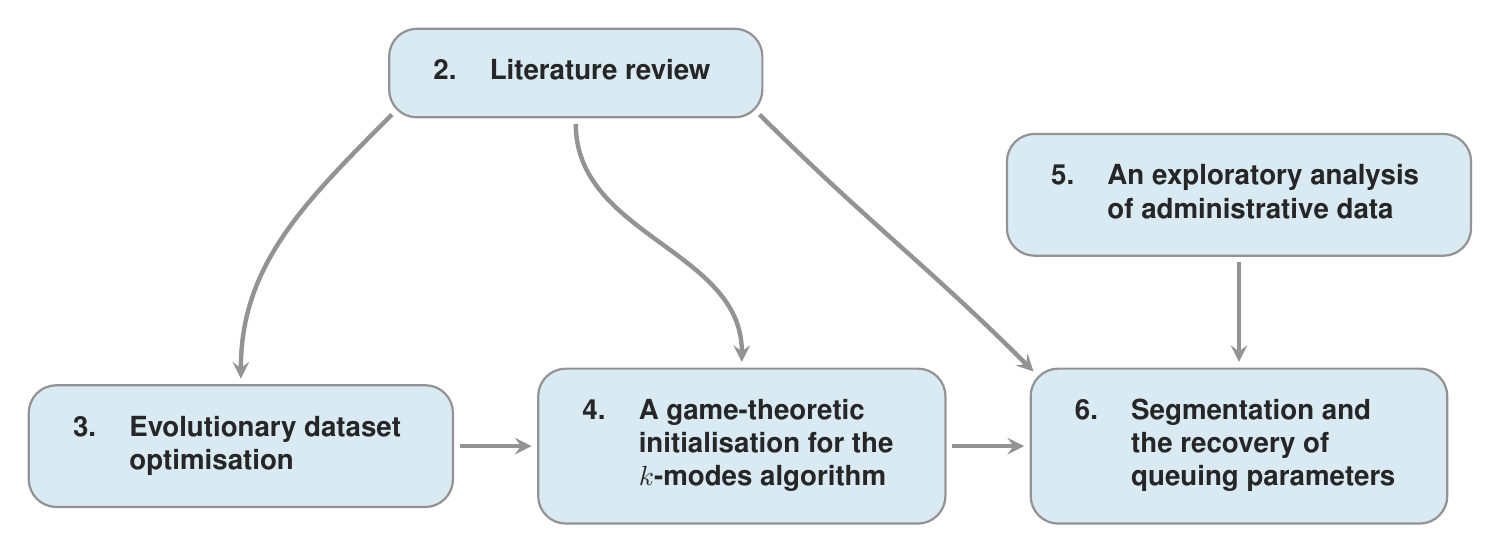
\begin{tikzpicture}

    %% Style settings

    \usefont{T1}{phv}{b}{n}\color{black!85}\selectfont
    \tikzstyle{chapter} = [%
        inner sep=1em,
        rounded corners=1em,
        draw=gray!85,
        thick,
        fill=blue!15,
        minimum height=3em,
    ]
    \tikzstyle{connection} = [%
        -stealth,
        ultra thick,
        shorten <=2pt,
        shorten >=2pt,
        gray!85,
    ]

    %% Nodes

    \node[chapter] (lit) {%
        \textbf{%
            \begin{tabular}{ll}
                2. & Literature review
            \end{tabular}
        }
    };

    \node[below=9em of lit, xshift=6em, chapter] (kmodes)
        {%
            \textbf{%
                \begin{tabular}{ll}
                    4. & A game-theoretic\\
                       & initialisation for the\\
                       & \(k\)-modes algorithm
                \end{tabular}
            }
        };
    
    \node[left=3em of kmodes, chapter] (edo)
        {%
            \textbf{%
                \begin{tabular}{ll}
                    3. & Evolutionary dataset\\
                       & optimisation
                \end{tabular}
            }
        };

    \node[right=3em of kmodes, chapter] (copd)
        {%
            \textbf{%
                \begin{tabular}{ll}
                    6. & Segmentation and\\ 
                       & the recovery of\\
                       & queuing parameters
                \end{tabular}
            }
        };

    \node[above=4em of copd, chapter] (data)
        {%
            \textbf{%
                \begin{tabular}{ll}
                    5. & An exploratory analysis\\
                       & of administrative data
                \end{tabular}
            }
        };


    %% Arrows

    \draw[connection, shorten <=-2pt]
        (lit.south west) to[out=225,in=90] (edo.north);
    
    \draw[connection] (lit.south) to[out=270,in=90] (kmodes.north);
    
    \draw[connection, shorten <=-2pt, shorten >=-2pt]
        (lit.south east) to[out=315, in=135] (copd.north west);

    \draw[connection] (edo.east) to (kmodes.west);
    
    \draw[connection] (kmodes.east) to (copd.west);

    \draw[connection] (data.south) to (copd.north);

\end{tikzpicture}

\end{document}
